% TODO: interpretability

What if machines can read our mind? 
If we can give a machine a few keywords and let the machine generate a sentence from these keywords, writing tasks could be made more efficient.
This is what autocomplete systems are trying to achieve. 
The way in which we choose the keywords is also important. 
Taking just the first or the last few words of a sentence as keywords usually does not capture the full meaning of the sentence.
For example, if someone wants to capture the meaning of \textit{'I live in Amsterdam'} in a few keywords, the words \textit{'live Amsterdam'} would probably be chosen. 
Thus, the keywords come from multiple places in the sentence. 
Therefore, autocomplete systems need to use more complex models to be more efficient and accurate. 

\section{Literature review}

\subsection{Autocomplete communication game}

\begin{figure}
    \centering
    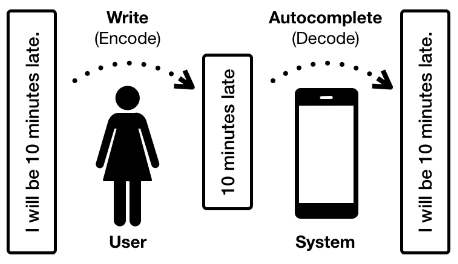
\includegraphics[width=.5\linewidth]{figs/autocomplete_game.png}
    \caption{Schematic overview of the communication game. Figure from \protect\shortciteA{autocomplete}.}
    \label{fig:autocomplete}
\end{figure}

The same autocomplete communication game is considered as in \shortciteA{autocomplete}. In this game, a human (called user) encodes a sentence into keywords. 
These keywords are then decoded by a machine (called system) to retrieve the full, initial sentence. 
A schematic overview is given in figure \ref{fig:autocomplete}. 
The communication game is successful if the retrieved sentence is the same as the initial sentence. 

More formally, a target sentence $x=(x_1, \dots, x_m)$ is communicated by a user through the keywords $z=(z_1, \dots, z_n)$. 
Note that $z$ is a subsequence of $x$. 
The system then tries to retrieve the target sentence by decoding the keywords. 
The target sentence is described by the keywords using encoding strategy $q_{\alpha}(z | x)$ and the system decodes the keywords by using decoding strategy $p_{\beta}(x|z)$. 

For a model to be efficient, the number of keywords needs to be as low as possible. 
In addition, for a model to be accurate, the probability of reconstructing $x$ from $z$ needs to be as high as possible. 
Therefore, a cost and a loss, respectively, can be defined:
\begin{equation}
    \label{eq:cost}
    \text{cost}(x,\alpha) = \mathbb{E}_{q_{\alpha}(z|x)} [\text{length}(z)]
\end{equation}
\begin{equation}
    \label{eq:loss}
    \text{loss}(x,\alpha,\beta) = \mathbb{E}_{q_{\alpha}(z|x)} [-\log p_{\beta}(x|z)]
\end{equation}

\subsection{Segmentation model}
\label{sec:segmentation}
% Why does a segmentation model work?

\paragraph{General idea.}
If there is a rod of length $n$, and we can cut this rod at every marker, how can we best find the maximal total value of the resulting pieces?
This is called the rod cutting problem.
The segmentation model gives a solution to the rot cutting problem. 
The segmentation model takes the scores of all pieces of the rod, called segments. 
Those segments can be of length 1, 2 or even $n$. 
With these scores, the model determines what the best possible segmentation is. 
To find the best segmentation and the probability of a segmentation, the model makes use of dynamic programming algorithms such as the Viterbi algorithm \shortcite{Viterbi} and the forward algorithm.
The segmentation model is essentially a simpler version of a hidden semi-Markov model \shortcite{hsmms}. 

\paragraph{Segmentation model for text.}
So how does the segmentation model work for text? 
If we have a sentence, e.g. \textit{'I will be late'}, we can use fence post indexing to represent a sentence as a rod which can be cut at the fence posts (see also figure \ref{fig:fencepost}).
The fence posts can also represent nodes in a directed acyclic graph (DAG). 
We can then draw edges between those nodes that represent segments. 
Those segments can be seen as (groups of) words. 
In figure \ref{fig:dag}, a DAG can be seen in which all the possible segments are showed. 
In the case of the autocomplete communication model described before, a segment is either kept or not.
Therefore, we can have one edge representing 'keep' and one representing 'do not keep', resulting in figure \ref{fig:dag2}.
If the pink edges are taken as 'do not keep' and the blue ones as 'keep', two possible segmentations can be seen in figure \ref{fig:segmentation} and \ref{fig:segmentation2}. 
Both segmentations result in the keywords \textit{'will be late'}. 

The score of a segmentation can be calculated by summing up all scores of its segments.
The assigned score of a segment can be visualized as a score matrix $A$ and has size $(m+1) \times (m+1)$. 
A segment, e.g. segment $i-j$, only has a score if it goes to a node further in the sequence, i.e. $i < j$.
Therefore, only the upper triangle of the matrix is used. 
This is denoted in figure \ref{fig:matrixA} by the gray squares.
The scores of the segmentations can then be used to calculate probabilities and to sample from a distribution over segments.

\begin{figure}
    \centering
    \begin{subfigure}[b]{0.45\textwidth}
        \centering
        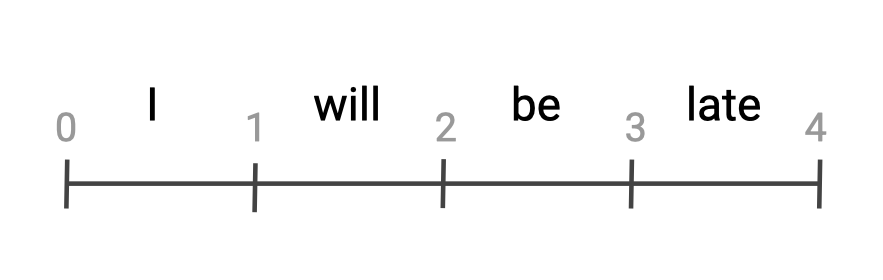
\includegraphics[width=0.9\textwidth]{figs/fencepost.png}
        \caption{Fence post indexing}
        \label{fig:fencepost}
    \end{subfigure}
    \hfill
    \begin{subfigure}[b]{0.45\textwidth}
        \centering
        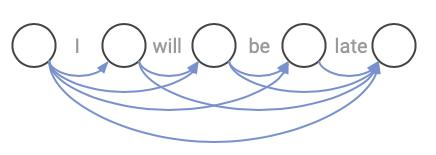
\includegraphics[width=\textwidth]{figs/segmentation1.jpeg}
        \caption{Possible segments in a DAG}
        \label{fig:dag}
    \end{subfigure}
    \hfill
    \begin{subfigure}[b]{0.45\textwidth}
        \centering
        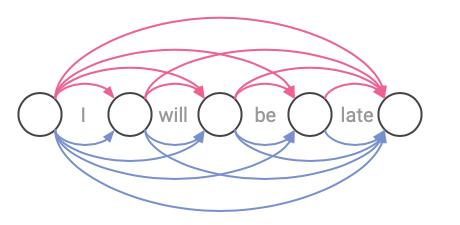
\includegraphics[width=\textwidth]{figs/segmentation2.jpeg}
        \caption{Possible segments in a DAG when each segment can either be true or false}
        \label{fig:dag2}
    \end{subfigure}
    \hfill
    \begin{subfigure}[b]{0.45\textwidth}
        \centering
        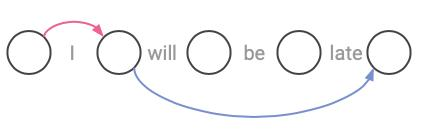
\includegraphics[width=\textwidth]{figs/segmentation3.jpeg}
        \caption{A possible segmentation}
        \label{fig:segmentation}
    \end{subfigure}
    \hfill
    \begin{subfigure}[b]{0.45\textwidth}
        \centering
        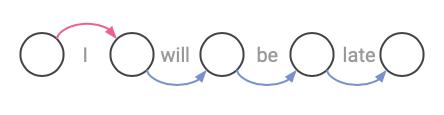
\includegraphics[width=\textwidth]{figs/segmentation4.jpeg}
        \caption{Another possible segmentation}
        \label{fig:segmentation2}
    \end{subfigure}
    \hfill
    \begin{subfigure}[b]{0.45\textwidth}
        \centering
        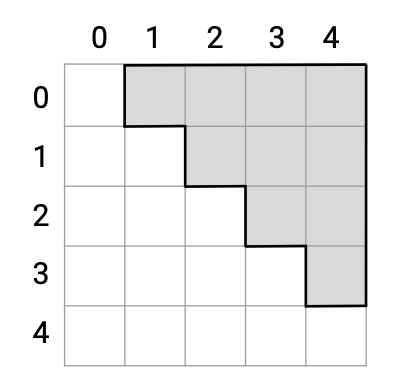
\includegraphics[width=0.6\textwidth]{figs/matrixA.png}
        \caption{Score matrix A}
        \label{fig:matrixA}
    \end{subfigure}
    \caption{Segmentation model}
    \label{fig:segmentation_model}
\end{figure}

\subsection{Structured latent variables}
% What is a latent variable?
A latent variable is variable that cannot be observed directly.
It can be used to capture some relevant property of a data point \shortcite{niculae2023discretelatentstructureneural}.
Since we cannot observe these variables, usually there are no labels available for them. 
Therefore, it is not possible to use supervised learning on them. 

% Structured discrete latent variables
\paragraph{Structured latent variables.}
A structured latent variable can be used when structure is useful for interpreting our data \shortcite{LatVar}. 
In the case of our autocomplete communication game, we try to recover the full sentence by inferring what is a good mask.
The mask determines what words are good keywords.
By adding the segmentation model, we make the latent variable structured, namely in the form of a segmentation.


% Monte Carlo gradient estimation
\paragraph{Score function estimator.}
Because our latent variable, the mask, is a discrete variable, which is also part of our training objective, we cannot calculate a gradient \shortcite{MCGE}.
However, the gradient is needed for optimization of the model. 
In the case a gradient cannot be calculated, we can use a score function estimator (SFE, \citeNP{paisley2012variational,rubinstein1976monte}) in combination with Monte Carlo estimation.
The SFE is also known as REINFORCE \shortcite{Williams1992}.

The SFE allows us to rewrite our gradient with respect to the parameters $w$ of the model,
\begin{equation}
    \nabla_w \mathbb{E}_{p_w(x)}[f(x)],
\end{equation}
to
\begin{equation}
    \mathbb{E}_{p_w(x)}[f(x)\nabla_w \log p_w(x)].
\end{equation}
For a derivation, see \shortciteA[p. 74]{niculae2023discretelatentstructureneural} for a general derivation or appendix \ref{app:gradients} for the specific case of our model. 
Adding Monte Carlo then results in:
\begin{equation}
    \label{eq:mc}
    \frac{1}{N} \sum_{n=1}^N f(\hat{x}^{(n)}) \nabla_{\theta} \log p_w(x),
\end{equation}
where $\hat{x}^{(n)} \sim p_w(x)$.

The SFE often has a high variance. 
This can influence training of the model negatively \shortcite{MCGE}.
It therefore is often used in combination with a control variate.
This control variate is a constant $c$ that is subtracted from the sample of the Monte Carlo estimator, rewriting equation \ref{eq:mc} in:
\begin{equation}
    \frac{1}{N} \sum_{n=1}^N f(\hat{x}^{(n)} - c) \nabla_{\theta} \log p_w(x).
\end{equation}
Because of this, the score function estimator has a lower variance. 
In addition, because the control variate is a constant, the gradient is not affected by this.

\section{Current research}
% Gap
% Research question: To what extend can a segmentation model help by selecting keywords for an auto-complete communication game?
% TODO: check references - are they relevant?
% into account for what?

Previous research did not take a structured model for autocompletion into account \shortcite{Bar-YossefZiv2011Cqa,autocomplete,SvyatkovskiyAlexey2019PACC}.
Since language is structured, a structured model, namely the segmentation model, can be more natural and effective than the current bit mask that is implemented in \shortciteA{autocomplete}.
Furthermore, previous work has shown that the prediction of segmentations can lead to better results than models that do not explicitly represent segments \shortcite{kong2016segmentalrecurrentneuralnetworks,conditionalRandomFields}. 
Therefore, in this research, we look at how a latent segmentation model can be used to retrieve keywords from a sentence. 
First, the autoencoder model used in \shortciteA{autocomplete} will be implemented. 
Then, the segmentation model will be implemented in the encoder of the previous model. 